\documentclass{article}
\usepackage[round]{natbib}

\usepackage[letterpaper,margin=1in]{geometry}
\usepackage{lineno}   %% <- no mathlines option
\usepackage{amsmath}  %% <- after lineno
\usepackage{etoolbox} %% <- for \cspreto, \csappto
\usepackage{amsfonts}
\usepackage{graphicx}
\usepackage{color}
\usepackage{url}
\usepackage{authblk}
\usepackage{bm}

\usepackage{setspace, caption}
\captionsetup{font=onehalfspacing} % Spacing in float captions

\usepackage{xr}
\externaldocument{supplement}

\DeclareMathOperator{\Var}{Var}
\DeclareMathOperator{\Cov}{Cov}
\newcommand{\aprcomment}[1]{{\textcolor{blue}{APR: #1}}}
\newcommand{\E}{\mathbb{E}}
\usepackage{xspace}
\newcommand{\moments}{\texttt{moments}\xspace}
\newcommand{\fwdpy}{\texttt{fwdpy11}\xspace}
\newcommand{\tskit}{\texttt{tskit}\xspace}

%% Patch 'normal' math environments:
\newcommand*\linenomathpatch[1]{%
  \cspreto{#1}{\linenomath}%
  \cspreto{#1*}{\linenomath}%
  \csappto{end#1}{\endlinenomath}%
  \csappto{end#1*}{\endlinenomath}%
}

\linenomathpatch{equation}
\linenomathpatch{gather}
\linenomathpatch{multline}
\linenomathpatch{align}
\linenomathpatch{alignat}
\linenomathpatch{flalign}

%\linenumbers

\title{Archaic introgression and the distribution
of shared variation under stabilizing selection}
\author[]{Aaron P. Ragsdale}
\affil[]{Department of Integrative Biology, University of Wisconsin--Madison, WI, USA}
\date{\today}

\begin{document}
\maketitle    


\begin{abstract}
    
    Many phenotypic traits are under stabilizing selection, which maintains a
    population's mean phenotypic value near some optimum. The dynamics of
    traits and trait architectures under stabilizing selection have bene
    extensively studied for single populations at steady state. However,
    natural populations are seldom at steady state. Instead, they are often
    structured in some way, and admixture and introgression events may be
    common, including over human evolutionary history. Because stabilizing
    selection results in selection against the minor allele at a
    trait-affecting locus, alleles from the minor parental ancestry will be
    selected against after admixture. Here, we show that the site-frequency
    spectrum can be used to model the genetic architecture of such traits,
    allowing for the study of trait architecture dynamics in complex
    multi-population settings. We use a simple deterministic two-locus model to
    predict the reduction of introgressed ancestry around trait-contributing
    loci. From this and individual-based simulations, we show that
    introgressed-ancestry deserts are enriched around such loci. When
    introgression between two diverged populations occurs in both directions,
    as has been inferred between humans and Neanderthals, the locations of
    introgressed-ancestry deserts will tend to be shared across populations. We
    argue that stabilizing selection for shared phenotypic optima may explain
    recent observations in which regions of depleted human-introgressed
    ancestry in the Neanderthal genome overlap with Neanderthal-ancestry
    deserts in humans.

\end{abstract}

\onehalfspacing

\section*{Introduction}

Genomic surveys of natural systems show that historical admixture among
diverged populations and closely related taxa commonly occurs
\citep{brandvain2014speciation, skoglund2015ancient, suvorov2022widespread} and
is widespread in primate \citep{tung2017contribution, sorensen2023genome} and
hominin \citep{wolf2018outstanding, peter2020100} evolution. Admixture is
therefore a frequent driver of phenotypic and molecular variation and can
contribute to the genetic architectures of complex traits. In humans, archaic
introgression from Neanderthals and Denisovans has attracted considerable
attention, including efforts to describe the historical processes leading to
observed distributions of introgressed DNA in present-day populations
\citep{prufer2014complete, villanea2019multiple, chen2020identifying} and the
contribution of introgressed variation to quantitative traits
\citep{sankararaman2016combined, wei2023lingering}.

Once introduced through admixture, introgressed alleles may be selected for or
against. Some introgressed haplotypes were likely positively selected in modern
\emph{Homo sapiens} (here, ``humans'') \citep{huerta2014altitude,
racimo2017signatures, enard2018evidence, gower2021detecting}, possibly due to
locally adaptive variation that provided fitness advantages as humans
encountered novel environments. Despite some cases of adaptive introgression,
most introduced alleles were likely to have been selected against in humans
\citep{harris2016genetic, juric2016strength, veller2023recombination}. Since
Neanderthal and Denisovan population sizes were relatively small for hundreds
of thousands of years, theory predicts they would have accumulated deleterious
variation at an increased rate. Introgressed haplotypes loaded with more
deleterious mutations would have been rapidly removed by selection after
admixture. Mapping the distribution of Neanderthal-introgressed haplotypes in
humans shows a reduction of Neanderthal-related ancestry in coding and
regulatory regions \citep{petr2019limits, telis2020selection,
yermakovich2023long}. These ``deserts'' of Neanderthal ancestry support the
hypothesis that introgressed functional alleles were selected against
\citep{sankararaman2014genomic, sankararaman2016combined}.

There is growing genetic evidence that humans reciprocally contributed to
Neanderthal genomes \citep{kuhlwilm2016ancient, hubisz2020mapping,
harris2023diverse, li2024recurrent}. This gene flow occurred tens to hundreds
of thousands of years prior to Neanderthal introgression in humans during the
global dispersal of modern humans around 60 ka. This is supported by early
\emph{H. sapiens} outside of African around 200--100 ka \citep{schwarcz1988esr,
grun2005u, harvati2019apidima, beyer2021climatic}, potentially overlapping with
Neanderthals and providing opportunities for early contacts. While estimates of
the genomic contribution of early humans to Neanderthals vary, around $6\%$ of
later Neanderthal genomes may trace through this admixture event
\citep{harris2023diverse}. Under a ``load'' model, if human-related haplotypes
carried fewer deleterious alleles due to their larger long-term effective
population size, human-introgressed DNA would have been favored in Neanderthal
genomes. The replacement of Neanderthal mitochondrial and Y chromosomes by
early human haplotypes appears to support this model of post-admixture positive
selection in the Neanderthal lineage \citep{posth2017deeply,
petr2020evolutionary}.

Models for selection against introgressed alleles are often based on load
arguments (that is, due to differences in the rate of accumulation of
unconditionally deleterious variation in populations of different sizes) or
hybrid incompatibilities \citep{muller1942isolating}. These models, founded in
population genetics theory, rarely take into account selection operating on
phenotypic traits or the relationship between genetic and phenotypic variation.
Many phenotypic traits are thought to be under stabilizing selection
\citep{sanjak2018evidence, sella2019thinking}, including gene regulation
\citep{gilad2006natural, hodgins2015gene, price2022detecting}. Because some of
the strongest signals of selection against Neanderthal-introduced alleles are
in regulatory regions \citep{sankararaman2014genomic}, stabilizing selection on
quantitative traits may be particularly relevant to the dynamics of functional
genetic variation after introgression among hominins.

Stabilizing selection acts to maintain the phenotypic distribution of a trait
near some optimum, which is achieved by reducing phenotypic variation
(Figure~\ref{fig:stab-sel}A). When the mean phenotype of the population is
close to the phenotypic optimum, classical models predict that the minor allele
at a trait-affecting locus is selected against, with allele-frequency dynamics
equivalent to underdominant selection \citep{robertson1956effect}. This has
proven to be a useful model for understanding genetic architectures of traits
under stabilizing selection in single-population settings
\citep[e.g.,][]{keightley1988quantitative, simons2018population,
hayward2022polygenic}.

\begin{figure}[tb!]
    \centering
    \includegraphics{../figures/stab_sel.pdf}
    \caption{
        \textbf{Additive genetic variance under stabilizing selection.}
        (A) Stabilizing selection acts to maintain phenotypic values of
        individuals in the population near some optimum. Throughout, we assume
        a Gaussian fitness function.
        (B) With low mutational variance ($V_M$), the expected additive
        genetic variance ($V_G$) is proportional to the
        population-scaled mutation rate. When $V_M$ is large so that
        mutational effects can be strong, $V_G$ is independent of the mutation
        rate. The stochastic house-of-cards model (Eq.~\ref{eq:SHC})
        interpolates these regimes, assuming steady-state dynamics
        \citep{burger1989much}. Expected $V_G$ computed using an SFS approach
        \citep[developed here using \moments,][]{jouganous2017inferring}
        matches simulations assuming no linkage between loci affecting the
        trait, which align closely with the stochastic house-of-cards
        approximation.
        Here $V_S=1$, $N_e=10{,}000$, the mutation rate
        $\mu=0.01$ (per haploid), and mutation effects are drawn from a normal
        distribution with mean zero and variance $V_M$.
    }
    \label{fig:stab-sel}
\end{figure}

In diverged populations, the genetic variation contributing to a trait under
stabilizing selection has a higher rate of turnover compared to neutral
evolution \citep{yair2022population}. We therefore expect a rapid divergence of
trait architectures and an accumulation of fixed differences in the human and
Neanderthal lineages at trait-contributing loci, even when the mean phenotype
in each population remains close to the same trait optimum. When a derived
allele at high frequency in one population is introduced to another population
in which it was previously absent, it will be at low frequency (if the
admixture proportion is low) and subsequently selected against. Likewise, if
the ancestral allele is reintroduced to a population fixed for a derived
allele, the ancestral allele will be at low frequency and will be selected
against. Selection acts against the introgressed allele in either case, whether
it is ancestral or derived and regardless of the historical relative sizes of
the populations involved. In concurrent work, \citet{veller2024stabilizing}
demonstrate this effect by deriving the expected decay of minor parental
ancestry under stabilizing selection after admixture. This prediction contrasts
with the population-genetics load model, in which haplotypes with fewer
deleterious variants (such as those from the population with larger historical
size) are favored after introgression in either direction.

In this article, we show that admixture between diverged populations results in
selection against the minor parental ancestry at loci contributing to a trait
under stabilizing selection. We develop a numerical approach based on the
site-frequency spectrum to predict genetic variation under complex demographic
scenarios, and which we use to partition predicted trait heritability by
introgressed and non-introgressed variation. Using simulations with linkage, we
demonstrate that deserts of introgressed ancestry form around
trait-contributing loci. When gene flow occurs bidirectionally, such deserts
will tend to overlap in location across populations. We argue that stabilizing
selection on shared trait optima may explain the overlap of introgressed
ancestry deserts in human and Neanderthal genomes after reciprocal
introgression, as has been recently observed \citep{harris2023diverse}.

\section*{Model and Methods}

We consider a polygenic trait for which an individual's additive genetic value
is the sum over all effects of alleles in their genome. For individual $i$,
\(G_i = \sum_l g_{l, i} a_l\), where $a_l$ is the effect size of the derived
allele at locus $l$, and \(g_{l,i}\in\{0,1,2\}\) is their genotype at that
locus (i.e., the number of derived alleles they carry at that locus). With
linkage equilibrium between trait-affecting loci, the expected additive genetic
variance is \(V_A = \sum_l 2p_l(1-p_l)a_l^2\), where $p_l$ is the allele
frequency at locus $l$. We ignore dominance and epistatic effects (often argued
to be a reasonable modeling choice, e.g., \citet{barton2002understanding,
zhang2002pleiotropic}), so that \(V_G = V_A\). We further ignore environmental
effects and noise \citep[under the assumption of additive environmental
effects, as in][]{lande1975maintenance, simons2018population}, so that only
genetic effects are considered.

Stabilizing selection acts to reduce phenotypic variation around the optimum
value $O$, typically set to zero, and we assume a Gaussian fitness function
(Figure~\ref{fig:stab-sel}A) so that relative fitness (relative to an
individual with optimal phenotype) is given by \(f(G_i | O,
V_S) = \exp{(-(G_i - O)^2 / 2 V_S)}\). $\frac{1}{V_S}$ is interpreted as the
strength of selection on the trait, so larger $V_S$ implies weaker selection.
For a population with mean phenotype at or very close to the optimum, the
mean fitness of the population [assuming a normal distribution of phenotypic
values in the population, \citep{turelli1994genetic, urban2013asymmetric}] is
\[\bar{w} \approx \int_{-\infty}^\infty
f(G | O, V_S) \mathcal{N}(O, V_G) dG =
\left(\frac{V_S}{V_S+V_G}\right)^{1/2},\]
so that as the genetic variance increases, population mean fitness decreases.

\subsection*{Mutation rates, effect sizes and genetic variance}

If all alleles contribute equally to the trait
with effect sizes \(\pm a\) occurring in equal proportion,
\citet{keightley1988quantitative} showed that the dynamics of $V_G$ can be
approximated with the recursion
\[V_{G,t+1} \approx V_{G,t}\left(1-a^2/2(V_S+V_{G,t})\right)
\left(1-1/2N_e\right) + 2 \mu a^2,\]
where $\mu$ is the per-haploid, per-generation rate of mutation. In the
large-population-size limit, this gives the well-known result for
steady-state additive genetic variance,
\[V_G \approx 4\mu V_S,\] provided \(V_G \ll V_S\).

Mutations will not generally all have the same effect size, but rather are
drawn from some distribution. Here, when modeling mutation effects as
non-constant, we assume effect sizes follow a normal distribution with mean 0
and variance $V_M$. When population sizes or effect sizes are small, drift
dominates the dynamics of $V_G$, and at steady state \citet{lande1976natural}
found \[V_G \approx 4 N_e \mu V_M.\] Interpolating between the drift- and
selection-dominated regimes,
\begin{align}\label{eq:SHC}
    V_G & \approx \frac{4 \mu V_S}{1 + \frac{V_S}{N_e V_M}}.
\end{align}
This, the ``stochastic
house-of-Cards'' (SHC) approximation (Figure~\ref{fig:stab-sel}B), was given by
\citet{burger1989much} and is discussed in detail in \citet[][Ch.
28]{walsh2018evolution}.

\subsection*{Approximating allelic dynamics via underdominance}

As initially shown by \citet{robertson1956effect} \citep[see
also,][]{keightley1988quantitative, simons2018population}, when the mean
phenotype of the population is close to the optimal phenotypic value,
stabilizing selection results in selection against the minor alleles at loci
contributing additively to the trait, with dynamics mirroring symmetric
underdominance. In general, for an allele at frequency $p$ with selection
coefficient $s$, the expected change in $p$ over one generation is
\begin{equation}
    \E[\Delta p] = sp(1-p).
\end{equation}

In our case, the selection coefficient $s$ depends on the strength of selection
on the trait $V_S$ and the effect size $a$, as well as the frequency of the
allele, so that
\begin{equation}
    s\approx -\frac{a^2(1-2p)}{2(V_S+V_G)} 
    = \frac{\left(p-\frac{1}{2}\right)a^2}{V_S + V_G}
    \approx \frac{\left(p-\frac{1}{2}\right)a^2}{V_S},
\end{equation}
when $V_G \ll V_S$. This model assumes linkage equilibrium between
trait-contributing loci. We note that LD is expected to be generated between
loci even in the absence of linkage \citep{bulmer1971effect}, and
\citet{negm2024effect} recently showed how to correct for its effect on the
selection dynamics of a focal allele.

Because $a^2/(V_S+V_G)$ is always positive for any $a\not=0$, we see that
selection pushes allele frequencies to zero if $p<1/2$ and to one if $p>1/2$,
resulting in symmetric underdominance. Details are shown in
Appendix~\ref{sec:underdominance}.

\subsubsection*{Computing expected genetic variance from the SFS}

We model allelic dynamics using the diffusion approximation, where the expected
change in mean allele frequency per generation is
\[\E[M_{\delta_p}] = E[\Delta p] \approx s p(1-p),\]
with $s$ defined above, and the expected change in variance of the allele frequency per
generation is
\[\E[V_{\delta_p}] \approx \frac{1}{2N_e}p(1-p).\]


We extended the \moments-based solution for the sample site-frequency spectrum
(SFS) \citep{jouganous2017inferring} to include underdominance with given
selection coefficient $s$ (Appendix~\ref{sec:moments-underdominance}). The
contribution of alleles with effect size $a$ to the total genetic variance
$V_G$ is found by computing the expected pairwise diversity from the SFS (with
sample size $n$, denoted $\Phi_n$), as
\[V_{G,a} \approx 2a^2\sum_{j=1}^{n-1} \frac{j(n-j)}{n(n-1)} \Phi_n(j|a,\mu_a) da.\]
Here, $\mu_a$ is the mutation rate of alleles with effect size $a$. Then
assuming a normal distribution of effect sizes for new mutations, the total
genetic variance is
\[V_G \approx \int_{-\infty}^\infty V_{G,a}\mathcal{N}(0,V_M).\]
$V_G$ can be computed periodically in this way to predict trajectories in
non-equilibrium settings (Figure~\ref{fig:one-pop}).

If $V_G$ is non-negligible compared to $V_S$, ignoring $V_G$ and using
$s=(p-1/2)a^2/V_S$ leads to deflated estimates of additive genetic variance
(Figure~\ref{fig:supp-one-pop}). When mutation rates are large so that $V_G$ is
not small compared to $V_S$, using $s=(p-1/2)a^2/(V_S+V_G)$ provides estimates
of $V_G$ that closely match simulations assuming free recombination between
loci (Figures~\ref{fig:toy-admixture} and
\ref{fig:one-pop-0.01}--\ref{fig:one-pop-0.1}). Because $V_G$ can vary over
time, this means that $s$ is no longer constant and can change due to factors
such as non-constant demography that increase or reduce $V_G$.

\begin{figure}[tb!]
    \centering
    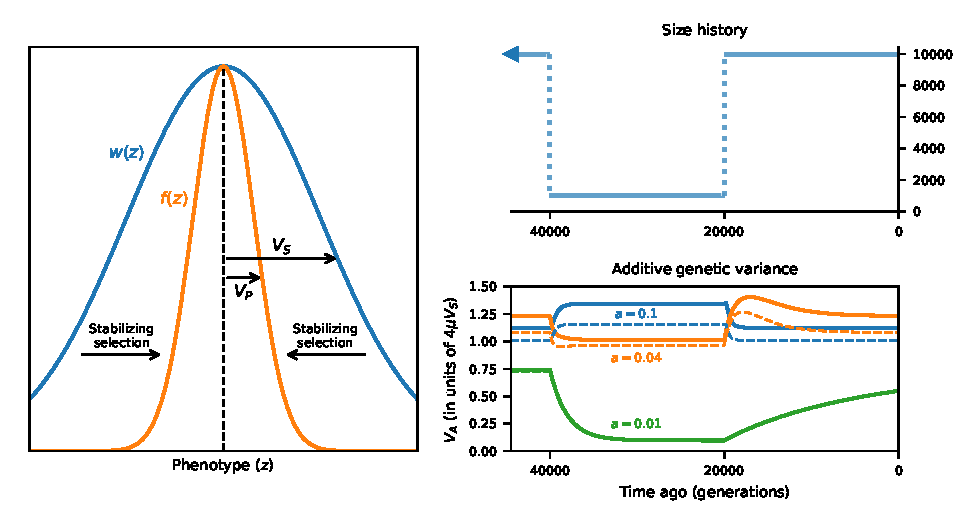
\includegraphics{../figures/one_pop.pdf}
    \caption{
        \textbf{Population size changes and additive genetic variance.}
        We used \moments to track expected genetic variance of a trait
        under stabilizing selection as the population changes size. (A) The
        population goes through a 10-fold size reduction, followed by a recovery.
        (B) All mutations have effect sizes $\pm0.01$, $0.04$, or $0.1$, with equal
        probability of being trait increasing or decreasing. Depending on the
        selection coefficient ($s\approx (p-1/2)a^2/V_S$) compared to $N_e$, $V_G$
        could increase or decrease after a sudden population size change.
        Predictions using \moments match simulations with free recombination
        between trait-affecting loci
        (Figures~\ref{fig:one-pop-0.01}--\ref{fig:one-pop-0.1}).
    }
    \label{fig:one-pop}
\end{figure}

\subsubsection*{Demographic history}

Our numerical solution for the SFS allows for non-constant population size
histories, population splits, continuous migration and admixture. Here, we
consider relatively simple scenarios involving population splits with
subsequent introgression events. We focus on parameter regimes relevant to
human-Neanderthal history. In a simple toy model (which is not meant to
perfectly match any particular known or inferred history, but instead
demonstrate the effect of reciprocal introgression following population
divergence) a population of size $N_e=10{,}000$ splits into two, one remaining
size $10{,}000$ and the other shrinking to size $1{,}000$. They remain isolated
for $2N_e$ generations (or 500 thousand years, assuming an average generation
time of 25 years) and then introgression occurs from one branch to the other,
contributing $5\%$ ancestry to the recipient population
(Figure~\ref{fig:toy-admixture}A,B).

The second model is meant to more closely resemble inferred human-Neanderthal
history, in which the ancestral population of size $N_e=10{,}000$ splits at 600
kya into the human and Neanderthal branches, with effective sizes $10{,}000$
and $2{,}000$, respectively. At 250 ka, an early human-to-Neanderthal
introgression contributes $5\%$ ancestry to Neanderthals. The human branch
shrinks to size $1{,}000$ 60 ka, followed by exponential growth to size
$20,000$ at present time. Neanderthals contribute $2\%$ ancestry to this
bottlenecked and expanding human population at 50 ka, after which they go
extinct (Figure~\ref{fig:human-neand-h2}A).

In each scenario, we tracked phenotypic variance and genetic variation to
compare simulations to model predictions. The trait optimum was kept at $0$ in
all populations (no optimum shift occurred), and the strength of selection
$V_S=1$ remains constant.

\begin{figure}[tb!]
    \centering
    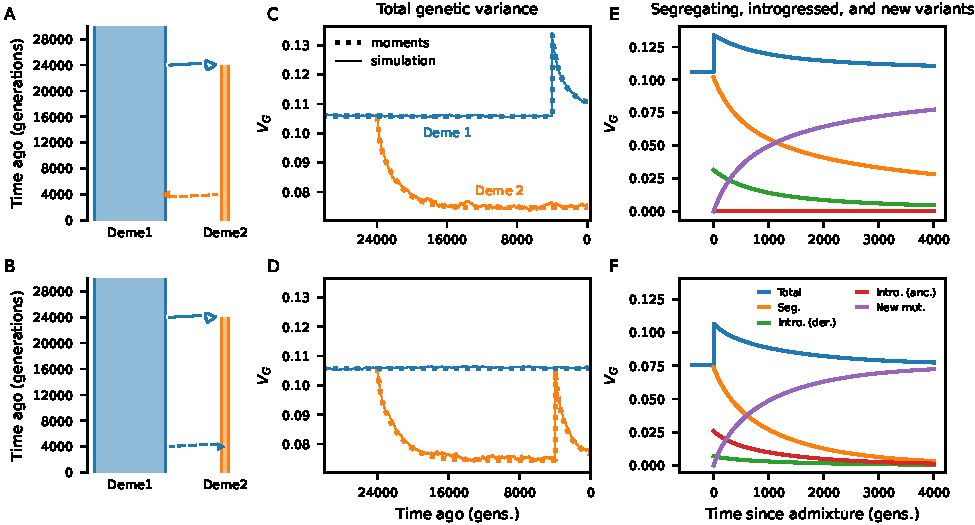
\includegraphics{../figures/reciprocal_admixture.pdf}
    \caption{
        \textbf{Genetic variance of a trait under stabilizing selection with
        multi-population demography.}
        (A,B) Two simple demographic models, in which Deme 1 has size 10,000
        and Deme 2 has size 1,000. In each scenario, we allow $5\%$ admixture
        from one deme to the other after begin isolated for 20,000 ($2N_e$)
        generations.
        (C,D) We compared predicted (additive) $V_G$ from the site-frequency
        spectra (using \moments) to simulations
        without linkage between trait-affecting loci. In Deme 2, $V_G$ decreases
        after divergence and population size reduction. After admixture in both
        directions, $V_G$ increases and then decays again toward levels at steady
        state. Predictions from \moments closely match observed $V_G$ in
        simulations.
        Here, mutations were drawn from a normal distribution of fitnesses
        with $V_M=0.0025$.
        Other parameters: $\mu=0.025$, $V_S=1$, and the optimal phenotype remained
        the same in each population.
        (E,F) Using \moments, we partitioned additive contributions to $V_G$ by
        mutations that were previously segregating in the focal population,
        introgressed variants (either derived or reintroduced ancestral alleles),
        and by new mutations since the time of admixture. In both demographic
        scenarios, introgressed variants contribute a substantial proportion to
        $V_G$, though it is primarily composed of introduced derived alleles when
        admixture is from the small to the large population, while primarily
        reintroduced ancestral alleles under the reverse direction of gene flow.
        In both cases, $V_G$ is increasingly due to new mutations and the genetic
        architecture of the trait turns over with time since admixture.
    }
    \label{fig:toy-admixture}
\end{figure}

\subsubsection*{Simulations with free recombination}

We compared our \moments-based predictions for $V_G$ in non-equilibrium
settings to simulations assuming linkage equilibrium as well as
individual-based simulations with recombination (next section). For both,
mutations occur at rate $\mu$ per haploid genome copy per generation, with
effects drawn from some distribution of mutation effects.

To simulate allele frequency changes under free recombination (assuming linkage
equilibrium between all trait-affecting alleles at all times), for each focal
segregating allele we integrated over possible genetic backgrounds contributed
by all other segregating alleles. Making the assumption that many alleles
contribute to the trait, the variance in genetic backgrounds is normally
distributed around the mean genetic value $E_{\tilde{G}}=\sum_l 2p_l a_l$ with
variance $V_{\tilde{G}}=\sum_l 2p_l(1-p_l)a_l^2$, where the sums omit the focal
locus. The expected change in frequency was then computed using the approach
outlined in Appendix~\ref{sec:underdominance} (without taking the first-order
Taylor series approximation for the exponentials). Allele counts in the next
generation were then binomially sampled with parameter $p+\E[\Delta p]$
independently for each allele.

\subsubsection*{Individual-based simulations with linkage}

To include the effects of linkage between multiple selected alleles or selected
and neutral alleles, we used \fwdpy \citep{thornton2019polygenic} to run
Wright-Fisher simulations under the demographic models described above. In
these simulations, we considered large (1 Morgan, or 100 Mb with a per-base
recombination rate of $10^{-8}$) chromosomes with a uniform recombination
landscape. Trait-affecting mutations were either uniformly distributed across
the chromosome (Figures~\ref{fig:linkage} and
\ref{fig:supp-low-VM}--\ref{fig:supp-high-VM}) or fell within functional
regions (Figures~\ref{fig:deserts} and
\ref{fig:deserts-high-VM}--\ref{fig:deserts-directional-B}). For the latter,
such regions were centered 2 Mb apart and were 100kb in size, so that there
were 50 evenly spaced regions across the chromosome. Mutation effect sizes were
drawn either as constant values $\pm a$, or from a normal distribution with
mutational variance $V_M$.

In these simulations, we tracked the empirical phenotypic variance (since there
is no simulated environmental effect, this is equivalent to $V_G$) in each
population each generation. We measured the effects of linked selection on
neutral introgressed ancestry using \tskit to analyze genealogical
information \citep{ralph2020efficiently}. To measure the reduction in
introgressed ancestry around introgressed variants (as shown in
Figure~\ref{fig:linkage}), we identified each locus with a fixed difference
between the parental populations at the time of admixture by preserving the
generation immediately preceding admixture. For such a locus, for each sample
we determined which (preserved) parental population its ancestry traced to at
varying distances from the selected locus. Ancestry proportions were then
averaged over each fixed difference. To measure proportions of introgressed
ancestry or probabilities of observed ancestry deserts (as in
Figure~\ref{fig:deserts}), we again used \tskit to average ancestry proportions
of the source population in 50 kb windows. Ancestry deserts were defined as
any such window with no ancestry inherited from the source population.

\subsection*{Data and code availability}

All code to run analyses, create figures, and compile this manuscript is
available at
\url{https://github.com/apragsdale/neanderthal_stabilizing_selection}.

\section*{Results}


\subsection*{Additive genetic variance after admixture}

We typically expect genetic variance to increase after introgression. The
amount that genetic variance increases depends on the allelic differences
accumulated between populations and the effects of those alleles. Assuming
linkage equilibrium, and ignoring dominance and epistasis, \(V_G=\sum_l
2p_l(1-p_l)a_l^2\). After admixture, with proportion $f$ contributed by the
population labeled 0 and $1-f$ by population 1, \(p_l = fp_{l,0} +
(1-f)p_{l,1}\). Plugging into the expression for $V_G$ and after a bit of
algebra (Appendix~\ref{sec:VG-admixture}), we can write the expected genetic
variance directly after admixture as
\[V_G = fV_{G,0} + (1-f) V_{G,1} + 2f(1-f)\sum_l F_{2,l} a_l^2,\]
where $F_2 = (p_0 - p_1)^2$ is the squared difference in allele frequencies at
a locus \citep{peter2016admixture}. This result is known
\citep[e.g.,][]{tufto2000quantitative}, showing that additive variance is equal
to that in the source populations weighted by their contributions, plus a term
that depends on the divergence at trait-affecting loci between the populations
weighted by the quadratic factor $2f(1-f)$. Notably, $V_G$ is expected to
increase only in the second generation after admixture, so that selection
against introgressed alleles is not immediate \citep{veller2024stabilizing}.
This effect is not captured by this expression.

$F_2$ at a given locus depends on the demographic history
relating the two populations and the effect size at the locus due to selection
on the trait. In the infinitesimal limit, involving many loci each of
vanishingly small effect, dynamics at a given locus will be approximately
neutral, so that $F_2$ depends only on demographic history. In this case,
\begin{align} \label{eq:VG-admixture}
    V_G & \approx f V_{G,0} + (1-f) V_{G,1} + 2f(1-f)\mathbb{E}[F_2] \sum_l a_l^2 \\
    \nonumber
    & = f V_{G,0} + (1-f) V_{G,1} + 2f(1-f)\mathbb{E}[F_2] L V_M,
\end{align}
where $L$ is the number of trait affecting loci and assuming $\E[a]=0$.


\begin{figure}[ht!]
    \centering
    \includegraphics{../figures/h2-per-SNP.pdf}
    \caption{
        \textbf{Allele contributions to heritability under human-Neanderthal
        reciprocal introgression.}
        (A) A simple model of divergence and admixture between humans and
        Neanderthals. Using \moments, we computed predicted $V_G$ over time,
        partitioned by variation that was introgressed vs. non-introgressed
        (Figure~\ref{fig:human-neand-VG}).
        (B-E) Predicted per-SNP contributions to genetic variance ($h^2$ per
        SNP) is plotted over the 50 thousand years following introgression.
        For non-introgressed variants, we also plot $h^2$ per SNP weighted by
        allele frequencies matching those of introgressed variants. These
        are shown for (B,C) Neanderthal-to-human introgression 50 kya,
        (D,E) human-to-Neanderthal introgression 250 kya, (B,D) $V_M=0.0025$,
        and (C,E) $V_M=0.0001$.
    }
    \label{fig:human-neand-h2}
\end{figure}

\subsubsection*{Predicted \bm{$V_G$} from the SFS}

Expected allele frequency differences ($F_2$) for selected alleles differ from
neutrality. For negative and underdominant selection, $F_2$ is reduced relative
to neutral expectations (Figure~\ref{fig:underdominance-F2}). Because analytic
solutions are unavailable for arbitrary evolutionary scenarios involving
multiple populations, we numerically solve for the expected joint distribution
of allele frequencies (the SFS) before and after admixture. This provides a
numerical solution for expected $V_G$, which can be tracked over time
(Methods). Comparing to simulations with free recombination between loci, we
observe close agreement with average $V_G$ at all times
(Figure~\ref{fig:toy-admixture}C,D). In the scenarios tested here, admixture
causes a sudden increase in $V_G$ followed by a fairly rapid return to
pre-admixture levels, which is recovered by our numerical approach.

Modeling the dynamics of genetic variance using the SFS lets us examine
contributions to $V_G$ from different classes of mutations, such as those at
different frequencies or arising at different times, and how those
contributions change over time. In particular, we may quantify the contribution
to $V_G$ from alleles that were already segregating in the recipient
population, those that were introduced through introgression, and new mutations
since the time of admixture (Figure~\ref{fig:toy-admixture}E,F). In many
scenarios of interest, in which populations are considerably diverged at the
time of admixture, genetic architectures will be largely unique in each
population. After mixing, previously segregating and introgressed alleles each
contribute to $V_G$ before going to fixation or loss, and the variance of the
trait is increasingly due to new mutations. 

Introgressed variation can initially make up a considerable portion of $V_G$,
with those alleles being either newly introduced derived alleles or
reintroduced ancestral alleles. The relative sizes of the two populations
impact the numbers of each, as derived alleles will accumulate more readily in
a population with smaller effective size. Nonetheless, the overall increase in
$V_G$ is similar in both directions of introgression, as the symmetric term
\(2f(1-f)\sum_l F_{2,l} a_l^2\) contributes in either case and can be much
larger than $f V_G$ from the source population
(Equation~\ref{eq:VG-admixture}).

\subsubsection*{Complex demography and partitioning heritability by origin of
alleles}

We used a historical model resembling inferred human-Neanderthal history
(Figure~\ref{fig:human-neand-h2}A) to explore the effects of population size
changes and reciprocal admixture on the additive genetic architecture of traits
under stabilizing selection. As expected (Figure~\ref{fig:toy-admixture}),
population contractions decrease $V_G$ as drift removes allelic diversity at
trait-affecting loci, while introgression increases $V_G$.

Because the genetic architectures considered here are purely additive, we can
track mutations in an admixed populations by whether they were previously
segregating, fixed or lost in either parental populations or if they arose as
new mutations since the time of admixture. Partitioning $V_G$ by contributions
from these different sets of mutations (Figure~\ref{fig:human-neand-VG}), we
find it is still primarily contributed by previously segregating,
non-introgressed mutations. $V_G$ due to existing mutations decays
monotonically over time and is rapidly replaced by new mutations.

The average contribution of introgressed vs. non-introgressed SNPs to $V_G$
(i.e., $h^2$ per SNP) can similarly by tracked over time. For the
human-Neanderthal demographic model and genetic architectures considered
here, the contribution per SNP of introgressed variants is initially lower than
that of non-introgressed variants. These contributions change over time,
depending on mutational variance, as well as demography
(Figure~\ref{fig:human-neand-h2}). When weighting $h^2$-per-SNP of
non-introgressed SNPs by matching to allele frequencies of introgressed
variants, relative contributions depend sensitively on evolutionary parameters
and the time since admixture.

\subsection*{The effects of linkage}

In the preceding sections, we found that approximating the dynamics of
trait-affecting alleles using an underdominance model
\citep{robertson1956effect} provides an excellent approximation of $V_G$ in
complex demographic scenarios. However, this relies on linkage equilibrium
between trait-affecting alleles. The inclusion of linkage can cause noticeable
distortions of expected $V_G$, so that Equation~\ref{eq:SHC} differs from
observed $V_G$ at steady state \citep{burger1989much, burger1994distribution,
walsh2018evolution}.

To investigate the effects of linkage, we used chromosome-scale
individual-based simulations \citep{thornton2019polygenic}. By varying the
mutation rate and the variance of effect sizes of new mutations, we included
scenarios ranging from low to high polygenicity and from weak to strong
selection on individual alleles. In this and the following sections, we
highlight two effects of linkage. First, we observe deviations of $V_G$ from
expectations under free recombination, which can be large for highly polygenic
traits. Second, selection on introgressed trait-affecting alleles results in a
reduction of introgressed ancestry in surrounding regions.

With linkage between two or more loci contributing to a trait under stabilizing
selection, linkage disequilibrium (LD) can develop between alleles. Notably,
stabilizing selection will lead to coupling LD between mutations of
opposite-signed effects and repulsion LD between those of same-signed effects
\citep{bulmer1971effect}. This is expected to decrease $V_G$. For lower
mutational variances ($2N_e V_M\approx1$, Figure~\ref{fig:supp-low-VM}), we
observe such a reduction in $V_G$. With low mutational input, and thus low
polygenicity, $V_G$ in individual-based simulations closely matches
expectations without linkage. With increasing mutation rate, $V_G$ is reduced
relative to those expectations. However, when the mutational variance is much
larger ($2N_eV_M\approx 50$), we see the reverse trend
(Figure~\ref{fig:supp-high-VM}). At low mutation rate, there is a close match
between observed $V_G$ and unlinked expectations, although simulated values are
slightly higher. As the mutation rate increases, $V_G$ increases to be
relatively much larger than expectations, rather than smaller.

The strength of the deviation of $V_G$ between models with and without linkage
depends on a number of factors. The total mutation rate affects not only the
polygenicity, with higher mutation rates causing higher number of segregating
alleles, but also the mean recombination rate between those alleles, as they
will be more or less densely distributed in the genome. The distribution of
effect sizes plays an important role, as seen by the opposite trends in $V_G$
relative to unlinked predictions (Figure~\ref{fig:supp-low-VM} vs.
Figure~\ref{fig:supp-high-VM}), which are most apparent with high mutation
rates, and thus high polygenicity. In such cases, there appear to be complex
dynamics involving the reduction in $V_G$ due to the Bulmer Effect
\citep{bulmer1971effect} and an increase in $V_G$ due to selective interference
\citep{hill1966effect}.

\begin{figure}[ht!]
    \centering
    \includegraphics{../figures/ancestry_reduction.pdf}
    \caption{
        \textbf{Reduced introgressed ancestry around alleles contributing to a
        trait under stabilizing selection.}
        Using a deterministic model
        (Equations~\ref{eq:system-p}--\ref{eq:system-D}), we model the
        frequencies of an introgressed trait-affecting allele and a linked
        neutral allele, initially absent from the recipient population so that
        their frequencies equal the introgression proportion ($f=0.05$).
        The neutral allele frequency is reduced at a rate that depends on
        the effect size of the selected allele and the probability of
        recombination between them. LD (as measured by $D=\Cov(p,q)$) decays
        to zero over time.
        (C) Alleles with strong effects are expected to result in a larger
        depletion of introgressed ancestry around the selected locus.
        (D,E) Compared to individual-based simulations, deterministic model
        predicts the dip in introgressed ancestry around trait-affecting loci,
        when the mutation rate is low, so that trait-affecting are sparsely
        distributed. When mutation rates (and thus polygenicity) are high,
        selected alleles are close together, so that selective interference
        is more pronounced and local ancestry is affected by multiple selected
        alleles.
    }
    \label{fig:linkage}
\end{figure}

\subsubsection*{Introgressed ancestry is reduced around introduced
trait-affecting alleles}

Because introgressed trait-affecting alleles are selected against as the minor
allele, introgressed ancestry segments in the regions surrounding the selected
alleles will also be removed due to linkage. The expected reduction in
introgressed ancestry will depend on the effect size of the linked
trait-affecting allele and the local probability of recombination. We first
consider a deterministic model for the frequency dynamics of introgressed
alleles (one selected, one neutral) with variable rate of recombination. This
simple model ignores the effects of drift and of interference between multiple
selected alleles.

We model a trait-affecting locus with a fixed difference between the two
parental populations, in which the derived allele may be fixed in either
population. At the functional locus, with admixture proportion $f$ from the
minor parental source, the initial frequency of the derived allele is either
$p_0=f$ or $p_0=1-f$. Over one generation, the expected allele frequency at the
selected locus is, to leading order in $s$,
\begin{align}\label{eq:system-p}
    p_{t+1} & = p_t - s p_t(1-p_t)(1-2p_t),
\end{align}
with \(s=a^2/2V_S\) for stabilizing selection.
As discussed above, if \(p_0<1/2\), \(p_t\rightarrow0\), and if
\(p_0>1/2\), \(p_t\rightarrow1\) as \(t\rightarrow\infty\).

We consider a neutral locus separated from the selected locus by recombination
probability $r$. Initially, the expected frequency of linked introgressed
ancestry is \(q_0=f\), which changes over time due to linked selection on the
trait-affecting allele. Letting \(D=\Cov(p,q)\) be the standard covariance
measure of LD between the alleles at the two loci, $q$ is expected to change as
\begin{align}\label{eq:system-q}
    q_{t+1} & = q_t - s D_t(1-2p_t).
\end{align}
Initially, \(D_0=\pm f(1-f)\), with \(D\) being
positive if \(p_0=f\) and negative if \(p_0=1-f\). LD between the loci changes
deterministically over time due to both selection and recombination, so that
\begin{align}\label{eq:system-D}
    D_{t+1} = D_t - r D_t - s D_t (1-2p_t)^2.
\end{align}
Together, this forms a
simple nonlinear system of equations for the deterministic change in allele
frequencies at the two loci and LD between them.

Using this model, we predicted the changes in introgressed allele frequencies
and LD after admixture for given effect size $a$ and recombination rate $r$
(Figure~\ref{fig:linkage}A,B). As expected, smaller effect sizes result in a
slower decay in introgressed ancestry frequency at both selected and linked
loci, and larger recombination rates more quickly decouple the linked ancestry
from the selected allele dynamics. Thus, the expected reduction in introgressed
ancestry is largest for larger effect sizes (Figure~\ref{fig:linkage}C), and LD
between the selected and linked neutral alleles is largest for neutral sites
closest to the selected allele (Figure~\ref{fig:supp-LD}).

We assessed the accuracy of the deterministic two-locus model using
individual-based forward-in-time simulations \citep{thornton2019polygenic}
under a simple demographic model (Figure~\ref{fig:toy-admixture}A), with
introgression fraction \(f=0.05\). We simulated a single chromosome of length 1
Morgan, with all mutations having effect sizes \(\pm a\) (\(a=0.02\) or
\(0.05\), in separate simulations), and we varied the total per-chromosome
mutation rate (\(\mu=0.001\), \(0.0025\) and \(0.01\)). For each
fixed-difference mutation in the parental populations, we determined the
average introgressed ancestry surrounding such loci $4{,}000$ generations after
admixture (Methods).

The deterministic model (Equations~\ref{eq:system-p}--\ref{eq:system-D})
provides a very good approximation when mutation rates are small. As the
mutation rate increases in these simulations, trait-affecting alleles are more
densely distributed along the chromosome. Deviations from the deterministic
model are due to multiple selected alleles affecting local introgressed
ancestry. For the highest mutation rate shown here, there can be many other
trait-affecting alleles within a 1 cM window around any focal SNP, distorting
dynamics away from predictions under the two-locus model.

\subsection*{Introgressed ancestry deserts are shared under stabilizing
selection and reciprocal introgression}

\begin{figure}[ht!]
    \centering
    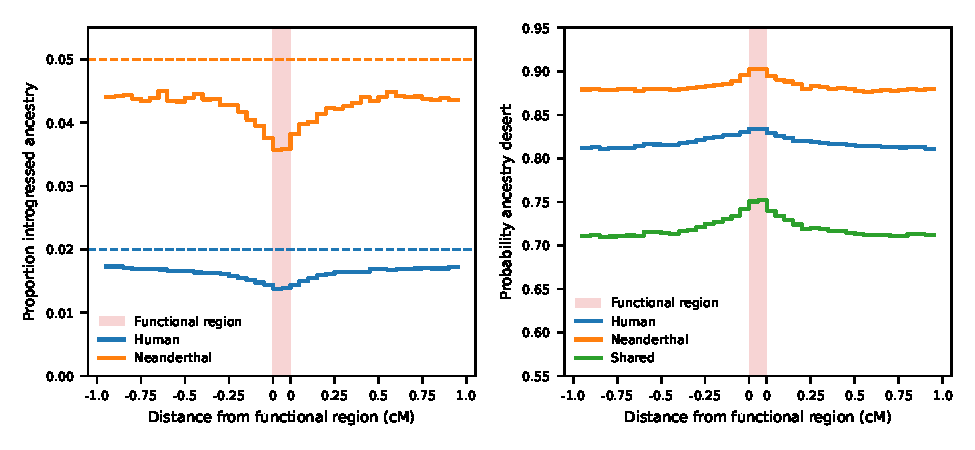
\includegraphics{../figures/introgression_deserts.SD_0.02.pdf}
    \caption{
        \textbf{Stabilizing selection causes an enrichment of introgressed
        ancestry deserts in functional regions.} (A) In chromosome-scale
        simulations under a demography with reciprocal migration between humans
        and Neanderthals (Figure~\ref{fig:human-neand-h2}A), stabilizing
        selection causes a chromosome-wide reduction of introgressed ancestry
        (below the $5\%$ and $2\%$ introgression proportions). This depletion
        is most pronounced in ``functional'' regions that allowed for
        trait-affecting mutations. (B) Introgressed ancestry deserts are
        more likely to occur in such functional regions, as are
        \emph{shared} deserts when compared across samples from humans and
        Neanderthals. In these simulations, $\sigma_M=0.02$ and $\mu=0.01$.
        Simulations with different mutational variances are shown in
        Figures~\ref{fig:deserts-high-VM}--\ref{fig:deserts-low-VM}.
        The pattern of shared deserts is not seen in simulations with
        directional selection (Figures~\ref{fig:deserts-directional-A}
        and \ref{fig:deserts-directional-B}).
    }
    \label{fig:deserts}
\end{figure}

As shown in the previous section, introgressed ancestry is reduced around loci
with trait-affecting alleles regardless of the parental population the derived
allele is present in. We should therefore expect to observe reductions in
introgressed ancestry at the same trait-affecting loci after gene flow in
either direction. If introgression occurs in both directions, regions of
reduced introgressed ancestry will coincide around such loci, and introgression
``deserts'' that appear due to selection against trait-affecting alleles will
tend to be shared.

To demonstrate this effect, we performed chromosome-scale simulations under a
model of reciprocal introgression between humans and Neanderthals
\citep[Figure~\ref{fig:human-neand-h2}A,][]{harris2023diverse}. Mutations
affecting a trait under stabilizing selection in each population occurred in
100 kb ``functional'' regions, spaced 2 Mb apart (Methods). Sampling
individuals from both the human and Neanderthal lineages, we observed the
average introgressed ancestry proportions were lowest within and surrounding
functional regions (Figure~\ref{fig:deserts}A). This corresponded to an
increased proportion of ancestry deserts within the functional regions
(Figure~\ref{fig:deserts}B). Functional regions also displayed an enrichment
of \emph{shared} ancestry deserts, with the probability of observing ancestry
deserts (either within a population or shared) decaying to background levels as
the distance from the functional region increases.

\section*{Discussion}

Many phenotypic traits are under stabilizing selection \citep{hodgins2015gene,
sanjak2018evidence, sella2019thinking}. This has motivated using stabilizing
selection around a shared optimum as a null model for the dynamics of alleles
affecting polygenic traits, including in multi-population settings
\citep{yair2022population}. Stabilizing selection on a trait results in
symmetric underdominant selection at trait-contributing loci
\citep{robertson1956effect, keightley1988quantitative}, that is, selection
against the minor allele. Some theoretical and simulation studies consider the
effect of population differentiation and migration on the genetic architecture
of a trait under stabilizing selection \citep[e.g.,][]{tufto2000quantitative,
yeaman2011genetic, yair2022population}, but most previous work has focused on
single population scenarios, often assuming steady state dynamics. Episodes of
admixture and introgression commonly occur in many species' evolutionary
histories, so understanding their effects on the architecture of complex traits
is needed.

Here, we have shown that a multi-population, non-equilibrium approach for the
site-frequency spectrum with underdominance can be used to model the additive
genetic variance of a trait under stabilizing selection. While this approach
ignores some biological relevancies, such as linkage between sites,
non-additivity and pleiotropy, it still provides important insights into the
dynamics of trait architectures. For example, we can readily decompose
contributions from alleles of different origins, either by source population or
mutation time. It may therefore be useful for understanding the contributions
of introgressed variants to complex traits, such as hominin-introgressed
mutations in humans \citep{reilly2022contribution, wei2023lingering}. In the
limited scenarios explored here, we find that the expected contributions of
introgressed variants to heritability are complicated even in the purely
additive case, depending on the distribution of effect sizes, demographic
history and the time since admixture (Figures~\ref{fig:human-neand-h2} and
\ref{fig:human-neand-VG}).

After admixture between diverged populations, the additive genetic variance of
a trait rapidly increases. The genetic variance after admixture depends on both
the existing genetic variances within the parental population and their
divergence at trait-affecting loci, measured by $F_2$
(Equation~\ref{eq:VG-admixture}) \citep[see also,][]{veller2024stabilizing}.
$V_G$ is then expected to decay fairly quickly to background levels. During
this process, introgressed and pre-existing trait-affecting alleles are
replaced by new mutations, turning over the genetic architecture of the trait
(Figure~\ref{fig:toy-admixture}).  Selection occurs against the minor alleles
at trait-affecting loci, so that introgressed alleles from the minor parental
ancestry, whether derived or reintroduced ancestral alleles, are selected
against (Figure~\ref{fig:linkage}).

Selection against introgressed alleles also removes linked introgressed
ancestry in the surrounding regions. Thus, introgressed ancestry deserts are
more likely to form at and around loci contributing to selected traits
(Figure~\ref{fig:deserts}). This process is symmetric, so that deserts tend to
form in the same regions under reciprocal introgression. When comparing
distributions of introgressed haplotypes in two diverged populations with
recent bi-directional gene flow, we should expect to see an overlap of deserts
in genomic regions contributing to traits under stabilizing selection.

The expected pattern of shared ancestry deserts under stabilizing selection
differs from models of both deleterious load and incompatibilities, providing
testable hypotheses. Load-based models predict that haplotypes that have
accumulated more deleterious mutations, e.g., from a population with small
long-term effective population size, will be selected against under either
direction of gene flow. Introgressed ancestry at a given selected locus will
decrease in frequency in one introgression scenario and increase in the other.
This may explain the replacement of MT and Y chromosome DNA in Neanderthals by
human haplotypes after early human-to-Neanderthal introgression and the absence
of such Neanderthal haplotypes in modern humans \citep{posth2017deeply,
petr2020evolutionary}, but does not broadly match observations across the
autosomal genome \citep{harris2023diverse}.

The classical model of Bateson-Dobzhansky-Muller incompatibilities (BDMIs)
\citep{bateson1909heredity, dobzhansky1936studies, muller1942isolating}
explains the accumulation of reproductive isolation through negative epistatic
interactions that are exposed in hybrids. \citet{muller1942isolating}
hypothesized that such BDMIs should most often form between distant or unlinked
loci, instead of within a single locus or tightly linked loci. Because theory
and experiments show that hybrid incompatibilities are resolved via selection
against the minor parental ancestry \citep{matute2020rapid, moran2021genomic},
ancestry deserts should form in different genomic regions, since different
incompatibility alleles are selected against depending on the parental ancestry
proportions. While both BDMI and stabilizing selection models predict selection
against introgressed alleles, an important distinction is that deserts due to
selection against incompatibility loci are not expected to overlap under
bidirectional gene flow. While there is little empirical data on the
distribution of BDMIs, studies point to interacting BDMI alleles being unlinked
\citep{presgraves2003fine, li2022imbalanced} and an asymmetry in the alleles
under selection in different introgression scenarios
\citep{maheshwari2011genetics, moran2021genomic}.

Finally, turning to the distribution of introgressed ancestry deserts in humans
and Neanderthals, \citet{harris2023diverse} found that regions of depleted
Neanderthal ancestry in humans overlap more than would be expected by chance
with regions lacking human-introgressed alleles in the Altai Neanderthal.
Human-introgressed ancestry in the Neanderthal genome is also depleted in
functional regions \citep{harris2023diverse}, as is well-documented in humans
\citep{sankararaman2014genomic, sankararaman2016combined}. 
\citet{harris2023diverse} propose that epistatic interactions between
introgressed alleles and the recipient backgrounds could drive these patterns,
which they interpret as evidence for the initial process of speciation between
humans and Neanderthals. However, the observation of shared ancestry deserts
does not match expectations under a classic model of BDMIs as described above.
Instead, at least some of the pattern may be due to stabilizing selection
acting on complex traits, such as gene regulation. Importantly, such
overlapping ancestry deserts are expected even when a trait is under
stabilizing selection for the same phenotypic optimal value. While the
underlying causes of selection on introgressed alleles in humans and
Neanderthals remain largely unknown, stabilizing selection provides a
well-grounded explanation for observed patterns that should be considered when
testing for epistasis, incompatibilities and adaptive introgression.


%\section*{Acknowledgements}
%\begin{itemize}
%    \item Lab members
%    \item Kevin Thornton
%    \item Bret Payseur
%\end{itemize}

\bibliographystyle{genetics}
\bibliography{manuscript}

\appendix
\section*{Appendix}

\section{Stabilizing selection results in selection on trait-affecting alleles
equivalent to symmetric underdominance} \label{sec:underdominance}

This result is well known and has been derived many times before. We include it
here for completeness. We consider a polygenic trait under stabilizing
selection, and we assume the mean phenotype of the population is close to the
optimal value (0), which will be the case if the optimum has not shifted
recently. Because many segregating loci are assumed to contribute to the
phenotypic variance of the trait, the phenotypic distribution is
well-approximated as normally distributed around the optimum:
\(f(G)=\frac{1}{\sqrt{2\pi V_G}} e^{-G^2/2V_G}\). We assume a Gaussian fitness
function, so that the fitness of an individual with genotypic value $G$ is
given by \(w(G)=e^{-G^2/2V_S}\).

For a derived allele (labeled 1) with frequency $p$, the expected change in
frequency over one generation due to selection (in general) is
\[\E[\Delta p]=p(1-p)\frac{w_{1\cdot}-w_{0\cdot}}{\bar{w}},\]
where \(\bar{w}\) is the mean fitness of the population, and marginal fitnesses
for the derived and ancestral alleles are
\[w_{1\cdot}=p w_{11} + (1-p)w_{01},\]
and
\[w_{0\cdot}=p w_{01} + (1-p)w_{00}.\]
Here, $w_{11}$, $w_{01}$, and $w_{00}$ are the relative fitnesses of
individuals who are homozygous for the derived allele, heterozygous, or
homozygous for the ancestral allele, respectively.

We partition an individual's genetic values into contributions from their
genetic background ($\tilde{G}$) and the focal locus: $G=\tilde{G}+xa$, where
$x\in{0,1,2}$.  We then integrate over genetic backgrounds to find the expected
fitnesses of each genotype. As described in SI section 2.1 of
\citet{simons2018population}, because each individual locus contributes a small
amount to $V_G$, $V_{\tilde{G}}\approx V_G$ and the fitness function is well
approximated as \(f(\tilde{G})=\frac{1}{\sqrt{2\pi
V_G}}e^{-\tilde{G}^2/2V_G}\). Then, mean fitness
\[
    \bar{w} = \sqrt{\frac{V_S}{V_S+V_G}},
\]
as shown in the main text, and
\[ 
    w_{11} \approx \int_{-\infty}^\infty f(\tilde{G}) w(\tilde{G} + 2a) d\tilde{G}
    = \bar{w}\exp{\left(\frac{-4a^2(1-p)^2}{2(V_S+V_G)}\right)},
\]
\[
    w_{01} \approx \int_{-\infty}^\infty f(\tilde{G}) w(\tilde{G} + a) d\tilde{G}
    = \bar{w}\exp{\left(\frac{-a^2(1-2p)^2}{2(V_S+V_G)}\right)},
\]
and
\[
    w_{00} \approx \int_{-\infty}^\infty f(\tilde{G}) w(\tilde{G}) d\tilde{G}
    = \bar{w}\exp{\left(\frac{-4a^2p^2}{2(V_S+V_G)}\right)}.
\]

Taking the first-order Taylor series expansion of the exponentials
($e^{-x}\approx1-x$, for small $x$) and combining terms,
\[
    \frac{w_{1\cdot} - w_{0\cdot}}{\bar{w}} \approx \frac{-a^2(1-2p)}{2(V_S+V_G)},
\]
demonstrating the result.

This same result can be found by considering a haploid model
\citep{negm2024effect}. While the selection coefficient takes an equivalent
form to underdominance, we note that the mechanism differs: selection acts
against the minor allele, rather than for the heterozygous genotype.

\section{Moment equations for over- and underdominance}
\label{sec:moments-underdominance}

For symmetric underdominance, the relative fitnesses of genotypes \(aa:Aa:AA\)
are \(1:1-t:1\). We consider any value of $s$ (positive or negative,
corresponding to either under- or overdominance); with stabilizing selection,
\(t=\frac{a^2}{2V_S}\), so that heterozygous individuals always have reduced
fitness compared to either homozygote.

We extended \moments \citep{jouganous2017inferring} to compute the sample
site-frequency spectrum \(\Phi_{\mathbf{n}}\) for one or more (up to five)
populations with sample sizes \(\mathbf{n}\). This provides a good
approximation for the distribution of trait-affecting allele frequencies across
multiple populations if the trait optimum is shared across populations and each
population's mean phenotype remains close to that optimum. This is expected to
be the case if there are no optimum shifts in any lineage.  Hardy-Weinberg
equilibrium is assumed at all loci. Accounting for optimum shifts in one or
more lineages would require a combination of direct and underdominant selection
\citep[e.g.,][]{hayward2022polygenic}, which we leave for future work.

We refer readers to \citet{jouganous2017inferring} for a detailed introduction
to the general moments-based framework for the dynamics of \(\Phi_\mathbf{n}\).
Here, we describe how underdominant selection changes \(\Phi\) over a single
generation. With symmetric underdominance, selection acts on heterozygotes. This
can be formulated as some proportion of heterozygotes failing to reproduce in a
given generation, with those selected lineages replaced by copies drawn from
the full population.

In a single population, we consider $n$ tracked lineages of which $i$ of those
carry the derived allele (\(\Phi_n(i)\) is thus the count of loci with $i$
observed derived alleles in a haploid sample of size of $n$). $i$ can increase
or decrease due to selection ``events''. Here, we assume $t$ is small enough so
that at most a single selection event occurs among the $n$ lineages in any
given generation. This is a reasonable approximation as long as $t$ is not
extremely large \citep{jouganous2017inferring, krukov2021taming} -- for
selection coefficients induced by stabilizing selection, this is typically a
safe assumption.

Two selective events can change $i$ to $i+1$ or $i-1$: (a) a tracked copy
carrying a derived allele is heterozygous (paired with an ancestral
allele-carrying copy), selected against, and then replaced by an ancestral
allele drawn from the rest of the population, so that \(i\rightarrow i-1\), or
(b) a tracked copy carrying the ancestral allele is paired with a derived
allele-carrying copy, selected against, and then replaced by a derived allele,
so that \(i\rightarrow i+1\). In both cases, we require drawing two additional
lineages to find the \(\Phi_n\) in the next generation, one for the diploid
pair and one for the replacement allele (i.e., \(\Phi_n^{t+1}(i)\) requires
\(\Phi_{n+2}^t\)). This results in an unclosed system of equations, and we use
a quadratic jackknife approximation to approximate \(\Phi_{n+2}\) from
\(\Phi_n\), as described in \citet{jouganous2017inferring}.

The expected increase and decrease of $\Phi_n(i)$ due to selection is found by
enumerating the sampling probabilities of each selective event. For case (a),
\(i\rightarrow i-1\) (i.e., \(\Phi_n(i)\) is reduced) with probability
\[t\frac{i(n-i+2)(n-i+1)}{(n+2)(n+1)}\Phi_{n+2}(i),\] and \(i+1\rightarrow i\)
(\(\Phi_n(i)\) increases) with probability
\[t\frac{(i+1)(n-i+1)(n-i)}{(n+2)(n+1)}\Phi_{n+2}(i+1).\] For case (b),
\(i\rightarrow i+1\) with probability
\[t\frac{(n-i)(i+2)(i+1)}{(n+2)(n+1)}\Phi_{n+2}(i+2),\] and \(i-1 \rightarrow
i\) with probability \[t\frac{(n-i+1)(i+1)i}{(n+2)(n+1)}\Phi_{n+2}(i+1).\]
These can be combined (with negative rates for the reduction of \(\Phi_n(i)\))
to describe the change of \(\Phi_n(i)\) for all \(0\leq i \leq n\).
Figures~\ref{fig:underdominance-validation-small-s}--\ref{fig:overdominance-validation}
show that this approach, implemented in \moments, is accurate compared to
discrete Wright-Fisher simulations.

\section{Additive genetic variance after admixture}\label{sec:VG-admixture}

Here, we derive the expected genetic variance after admixture between two
source populations (Equation~\ref{eq:VG-admixture}). Suppose two population
(labeled 0 and 1) diverged some time in the past and then admix in proportions
$f$ and $1-f$.

Assuming random mating and no linkage, dominance or epistasis (so \(V_G=V_A\)),
\[V_G = \sum_l 2p_l(1-p_l)a_l^2 = \sum_l \pi_l a_l^2,\]
where $\pi$ denotes expected pairwise diversity.
At a given locus (dropping the $l$), after admixture the allele frequency is
\[p=f p_0 + (1-f) p_1,\]
so that
\begin{align*}
    2p(1-p) & = 2(f p_0 + (1-f) p_1)(1 - f p_0 - (1-f) p_1) \\
    & = f^2 2p_0(1-p_0) + (1-f)^2 p_1(1-p_1) + 2f(1-f) (p_0(1-p_1) + p_1(1-p_0)) \\
    & = f^2 \pi_{0,0} + (1-f)^2 \pi_{1,1} + 2f(1-f)\pi_{0,1}.
\end{align*}
Here, $\pi_{i,j}$ is the expected pairwise diversity between two samples, one
drawn from population $i$ and the other from population $j$. If $i=j$, this is
pairwise diversity within a single population.

Plugging into the definition for $V_G$, we get after admixture
\[V_G = f^2 V_{G,0} + (1-f)^2 V_{G,1} + 2f(1-f)\sum_l \pi_{0,1,l}a_l^2.\]
We can write $\pi_{0,1}$ at a given locus in terms of $\pi_{0,0}$, $\pi_{1,1}$,
and $F_2(0,1)=(p_0-p_1)^2$, a measure of single-locus allele frequency
differentiation \citep{peter2016admixture}. Then
\[\pi_{0,1} = F_2(0,1) + \frac{1}{2}\pi_{0,0} + \frac{1}{2}\pi_{1,1},\]
and
\begin{align*}
    V_G & = f^2 V_{G,0} + (1-f)^2 V_{G,1} + 2f(1-f)\sum_l \left[F_{2,l}(0,1)
    + \frac{1}{2}\pi_{0,0} + \frac{1}{2}\pi_{1,1}\right] a_l^2 \\
    & = f^2 V_{G,0} + (1-f)^2 V_{G,1} + 2f(1-f)\left[\frac{1}{2}V_{G,0} 
    + \frac{1}{2}V_{G,1} + \sum_l F_{2,l}(0,1)a_l^2\right] \\
    %& = \left(f^2 + f(1-f)\right) V_{G,0} + \left((1-f)^2 + f(1-f)\right)V_{G,1}
    %+ 2f(1-f) \sum_l F_{2,i}(0,1)a_l^2 \\
    & = f V_{G,0} + (1-f)V_{G,1} + 2f(1-f)\sum_i F_{2,l}(0,1)a_l^2.
\end{align*}

\end{document}
